% Thomas Bernardi
% University of Washington
% HLIN501 Study Guide
% November 2017

\documentclass[10pt]{article}
\usepackage[T1]{fontenc}
% \usepackage{babel}
\usepackage[margin=1in]{geometry}
\usepackage{parskip}
\usepackage{amsthm}
\usepackage{amsmath}
\usepackage{tabularx}
\usepackage{graphicx}
\usepackage{enumitem}
\graphicspath{ {./graphs/} }
\usepackage[noend]{algorithmic}
\usepackage{amsmath, amsfonts, amsthm, amssymb} 
\usepackage{listings}

\theoremstyle{definition}
\newtheorem{definition}{Definition}[section]
\newtheorem{theorem}{Theorem}[section]
\title{Colocolo\\\large Optimizations on Ocelot, a Relational Logic Solver in Rosette}
\date{March 2019}
\author{Thomas Bernardi, Altan Haan}

\DeclareMathOperator{\bigdot}{\bullet}

\begin{document}
	\maketitle

  \section{Introduction}

  \paragraph{Ocelot.} Ocelot is an embedding of relational logic, including some of Alloy, in Rosette. It was originally aimed for use in MemSynth, a tool for reasoning about memory consistency: which is the problem of defining how parallel threads can observe their shared memory state \cite{bornholdt17}. As such, a couple of optimizations that could have been implemented were not because they would not have had much effect on the type of problems that MemSynth would present. In particular, Ocelot did not implement skolemization or reduction to CNF for SAT (it simply sends queries to Rosette's default solver, Z3).

  \paragraph{Problem Statement.} Can these two optimizations, skolemization and translation to CNF, bring significant performance improvements to Ocelot?
  
  \paragraph{Our Approach} Colocolo extends Ocelot to include these two optimizations. We build on top of Ocelot's existing engine and implement the optimizations based on reference implementations from Kodkod \cite{torlak07}, the current backend for Alloy.

  \section{Skolemization}\label{sec:skolems}
  In this section we provide a high level description of the implementation details of skolemization. To distinguish between the syntax of quantifiers and their semantics we introduce two new terms:\\
  \theoremstyle{definition}
  \begin{definition}[Weak quantifier]
      A \textbf{weak quantifier} is one that \emph{semantically} acts as an existential quantifier (i.e. $\exists$ and $\neg \forall$).
  \end{definition}

  \begin{definition}[Strong quantifier]
      A \textbf{strong quantifier} is one that \emph{semantically} acts as a universal quantifier (i.e. $\forall$ and $\neg \exists$).
  \end{definition}

  Skolemization is a transformation that moves weak quantifiers to the highest syntactic level by replacing weakly quantified variables with functions (or relations in the case of alloy). Skolemization relies on a key second order equivalence:

  \begin{equation} \label{eqv1}
      \forall x \exists y~.~P(x, y) \Leftrightarrow \exists f \forall x~.~P(x, f(x))
  \end{equation}

  where $f(x)$ is a function (relation) that maps $x$ to $y$. Intuitively this is translating between ``forall $x$ there exists a $y$ such that $P(x, y)$'' into ``there exists a function $f : x \rightarrow y$ such that, forall $x$, $P(x, f(x))$.'' This is useful because the existence of an $f$ that satisfies the subformula is semantically equivalent to the satisfiability of the subformula if $f$ is a symbolic constant sent to the solver.

  In the case of bounded model checking (in both Kodkod and Ocelot), this significantly reduces formula size. Suppose we have the universe $\{A_1, \dots, A_n\}$. Considering the formula from our equivalence \ref{eqv1}, $\forall x \exists y~.~P(x,y)$ would get translated as follows:

  Without skolemization:
  \begin{equation} \label{woskolem}
      \bigwedge_{i=1}^n\bigvee_{j=1}^n P(A_i, A_j)
  \end{equation}

  With skolemization:

  \begin{equation} \label{wskolem}
      \bigwedge_{i=1}^nP(A_i, f(A_i))
  \end{equation}

  \subsection{The Algorithm}

  \theoremstyle{definition}
  \begin{definition}[Declaration]
      A \textbf{declaration} allows us to define variables in terms of other expressions (and all declarations can eventually be traced back to relations in the universe). A declaration contains a \textbf{variable}, a \textbf{multiplicity}, and an \textbf{expression}.

      \begin{center}
          \begin{tabular}{c c c c}
              $x$ & : & some & $E$ \\
              variable & & multiplicity & expression
          \end{tabular}
      \end{center}
  \end{definition}

  An weak quantifier extends the current scope with new bindings as defined in its \textbf{declarations}. For each of these \textbf{declarations} $d := v~:~m~R$, skolemization does the following:

  Assume $S_\forall$ is a list of all strongly quantified variables that are currently in scope.

  \begin{itemize}
      \item Define the \textbf{skolem relation}, $\textsf{R}_v$ of arity $\text{size}(S_\forall) + \text{arity}(v)$ (every element of $S_\forall$ should be unary).
      \item Define our \textbf{skolem expression} $\textsf{E}_v$ which will replace every occurrence of $v$ further down the AST.
      \item Approximate an \textbf{upper bound} for the \textbf{skolem relation}.
      \item Calculate \textbf{domain constraints} that ensure the ``inputs'' to $\textsf{R}_v$ are constrained in the same way that their corresponding universally quantified variables are---store these, these will be conjuncted with the formula on the way up the AST once there are no more existential quantifiers. Specifically, these constraints encode multiplicity information that relational bounds cannot infer.
      \item Add \textbf{range constraints} to the formula to ensure that the ``outputs'' of $S$ are constrained in the same way as $v$.
  \end{itemize}

  \subsubsection*{Skolem Expression}

  The \textbf{skolem expression}, $\textsf{E}_v$, is what actually replaces $v$. It is the result of joining each non-skolem $a_i \in S_\forall$ with the $\textsf{R}_v$, or $\textsf{E}_v := f~S_\forall~\textsf{R}_v$ where $S_\forall$ is interpreted as a list $[a_1,\dots,a_n]$ sorted by order of declaration, and $f$ is defined as follows:
  \begin{align*}
      f~[]~X& = X\\
      f~a_i::L~X& = f~L~a_i\textbf{.}X
  \end{align*}

  \subsubsection*{Upper Bound}
  At the moment, Colocolo assumes all quantified variables will be quantified over sets. This way, the upper bound of the \textbf{skolem relation} is simply the cross product of the upper bound of each strongly quantified variable (in order of declaration), together with the upper bound of $R$ in the last position.

  \subsubsection*{Domain Constraints}

  Suppose $R$ is of arity $n$. We call $\textsf{U}$ the universe. Let $I_v = \textsf{R}_v.\textsf{U} \dots \textsf{U}$ where $\textsf{U}$ is joined to $\textsf{R}_v$ $n$ times. Let the $i$th declaration $a_i~:~m_i~R_i$ be the declaration that binds the $i$th variable, $a_i \in S_\forall$. Let $k = \text{length}(S_\forall)$. Our domain constraint is:
  $$I_v ~ \texttt{in} ~ \{a_0~:~m_0~R_0, \dots, a_k~:~m_k~R_k~\vert~\top\}.$$

  Note the expression $\{a_0~:~m_0~R_0, \dots, a_k~:~m_k~R_k~\vert~\top\}$ defines a $k$-ary relation where the $i$th element obeys the $i$th \textbf{declaration} with no other constraints (any relation satisfies $\top$).

  The domain constraints for each subformula in the skolemized formula are lastly conjuncted together at the top level to form the final domain constraint for the whole formula.



  \subsubsection*{Range Constraints}
  Our range constraint is simply $(\textsf{E}_v ~\texttt{in}~R)\land(m~\textsf{E}_v)$. Let $f' := \textsf{skolemize}(f[\textsf{E}_v / v])$ in $Qv~:~m~R \mid f$ where $Q \in \{\exists, \neg \forall\}$. When our quantifier is $\exists$ the skolemized (sub)formula becomes $(\textsf{E}_v ~\texttt{in}~R)\land(m~\textsf{E}_v) \land f'$, otherwise when $Q$ is $\neg \forall$ we skolemize to $[(\textsf{E}_v ~\texttt{in}~R)\land(m~\textsf{E}_v)] \to f'$.

  \subsection{An example}
  Let $A$ and $B$ be relations of arity $n$ and $m$ respectively, and let $P$ be a predicate on $A\times B$. Suppose we wish to skolemize the formula
  \[\forall x : \texttt{one}\: A. \: \exists y : \texttt{some}\: B \mid P(x,y).\]
  We first traverse through the universal quantification of $x$, adding $x : \texttt{one}\: A$ to $S_\forall$. Next we reach the existentially quantified $y$. Following the above procedure, we define $\textsf{R}_y :_{m + 1} [\{\langle \rangle\}, U(A)\times U(B)]$, where $U(X)$ gives the upper bound on a relation $X$. We can then define the domain constraint
  \[\textsf{D}_y := \textsf{R}_y \bigdot\limits_{i = 1}^m \textsf{U}~\texttt{in}~\{x : \texttt{one}\: A \mid \top\},\]
  along with the skolem expression $\textsf{E}_y := x.\textsf{R}_y$. Note that $\textsf{R}_y .\bigdot\limits_{i = 1}^m$ means left-associatively joining \textsf{U} to $\textsf{R}_y$ $m$ times. Lastly, our range constraint is $(\textsf{E}_y~\texttt{in}~\texttt{some}~B)$. As the quantifier is just an $\exists$, our skolemized subformula becomes $(\textsf{E}_y ~ \texttt{in}~\texttt{some}~B) \land P(x, \textsf{E}_y)$. Conjuncted with the top level domain constraints, we obtain the total skolemized formula
  \[\textsf{R}_y \bigdot\limits_{i = 1}^m \textsf{U}~\texttt{in}~\{x : \texttt{one}\: A \mid \top\} \land [(\textsf{E}_y ~ \texttt{in}~B) \land (\texttt{some} ~\textsf{E}_y)] \land P(x, \textsf{E}_y).\]
  Replacing $\textsf{E}_y$ with $x.\textsf{R}_y$, we get our final skolemized formula
  \[\textsf{R}_y \bigdot\limits_{i = 1}^m \textsf{U}~\texttt{in}~\{x : \texttt{one}\: A \mid \top\} \land [(x.\textsf{R}_y ~ \texttt{in}~B) \land (\texttt{some} ~x.\textsf{R}_y)] \land P(x, x.\textsf{R}_y).\]

  \section{Translation to SAT}
  For Colocolo, we attempted to implement an optimized translation from arbitrary (quantifier-free) first-order boolean formulas to a CNF-SAT instance. In particular, we relied on Rosette's internal (symbolic) boolean AST representation, which we descended recursively and applied the following transformation rules:
  \begin{equation}\label{transand}
    \bigwedge_{i=1}^n F_i \leadsto \left(\bigwedge_{i=1}^n [\tilde{F}_i \lor \neg o]\right) \land \left(o \lor \bigvee_{i=1}^n \neg\tilde{F}_i\right),
  \end{equation}
  \begin{equation}\label{transor}
    \bigvee_{i=1}^n F_i \leadsto \left(\bigwedge_{i=1}^n [\neg\tilde{F}_i \lor o]\right) \land \left(\neg o \lor \bigvee_{i=1}^n \tilde{F}_i\right).
  \end{equation}
  In these translations, $o$ is a fresh auxiliary variable that is true if and only if the original $n$-ary formula is true, and $\tilde{F}_i$ represents the corresponding auxiliary variable produced by recursively applying the rule to $F_i$. Note that both (\ref{transand}) and (\ref{transor}) are translation rules used by Kodkod internally.

  In the process of translating, we also encode each original boolean variable and new auxiliary variable as an integer (with negative literals represented as the negation of the integer representation of the variable). Lastly, the instance was translated into DIMACS format and sent to Lingeling, a fast SAT solver \cite{biere17}.

  \section{Results}
  \subsection{Implementation Challenges}

  \paragraph{Skolemization.} While skolemization seems like it should be a simple algorithm, it contains many nuances in the context of relational logic. The largest challenge was translating these details from Kodkod's implementation to work with Ocelot's AST. We found that the best way to understand Kodkod's implementation was to create a mathematical representation as described in Section \ref{sec:skolems}. Once we had this, implementing it in Ocelot was relatively straightforward.

  \paragraph{CNF-SAT Translation.} During our implementation of the optimized CNF-SAT translation scheme, we encountered some performance difficulties due to the usage of Racket lists, which are linked lists with poor asymptotics. We fixed this slightly by using smarter list merging functions, although more improvements are definitely possible. A non-negligible bottleneck with our performance under this optimization can probably be alleviated using smarter data structures. 

  \subsection{Benchmarks}

  Since we implemented a few optimizations on top of Ocelot, we are mainly interested in what sort of performance improvement we may have gotten. We are interested in both the overall improvement (time to solve an Ocelot problem), as well as performance of our final SMT/SAT query. To evaluate our optimizations, we translated a supported subset of the standard benchmarks/examples bundled with Kodkod, which are written in Java and use the Kodkod internal representation for problems. We ran the benchmarks over all combinations of optimizations, and recorded the total time, solver time, and whether or not the SAT solver returned within a 30-second time limit. We had difficulty implementing a time limit for Rosette's internal solver, so we did not impose one.


  \subsubsection{Meow: Compiling Kodkod to Ocelot}
  In order to translate Kodkod benchmarks into Ocelot/Colocolo, we wrote \emph{Meow} in Java, a compiler from Kodkod ASTs into equivalent problem instantiations in Ocelot/Colocolo.
  \paragraph{Graph structure.} Internally, Kodkod represents its formulas and expressions as nodes in a DAG, rather than a tree. This node sharing is crucial to Kodkod's internal notion of equality between relations (and nodes in general), and additionally improves memory performance. This means the translation into Colocolo cannot simply inline each node. To address this, we cached the Kodkod nodes during the graph traversal, and declared them in the compiled output in a topologically sorted order (where incoming edges represent syntactic children).

  \paragraph{Ocelot limitations.} During our benchmark compilation, we discovered some limitations of Ocelot that went beyond the scope of our project. In particular,
  \begin{itemize}
    \item Ocelot currently has no support for integers, which Kodkod supports through extensive bit-blasting.
    \item Ocelot has difficulties with higher-arity declarations in quantified formulas. In particular, Ocelot assumes all declarations to be unary, with \texttt{one} multiplicity.
    \item Some relational operators are missing from Ocelot, such as relational override and if-then-else.
  \end{itemize}
  To deal with these restrictions, we only used benchmarks that did not utilize any of the mentioned features.
  
  
  \subsubsection{Benchmark Results}

  Figure \ref{fig:averages} is enough to get an idea of the effects of each optimization on performance but we included a detailed graph in Figure \ref{fig:total} to show that that there there are some cases where certain optimizations perform contrary to the averages shown in Figure \ref{fig:averages}.

  Our best (and really only) performance improvement is when we use skolemization, where we get a $2.7\times$ speedup in total runtime and $4.1\times$ speedup in solver runtime. As discussed above, this is most likely due to the significant decrease in formula size we get when we apply skolemization. Note that the SAT solver time includes the time spent translating to CNF in Rosette.

    \begin{figure}[h]
      \centering
      \begin{minipage}{.5\textwidth}
        \centering
        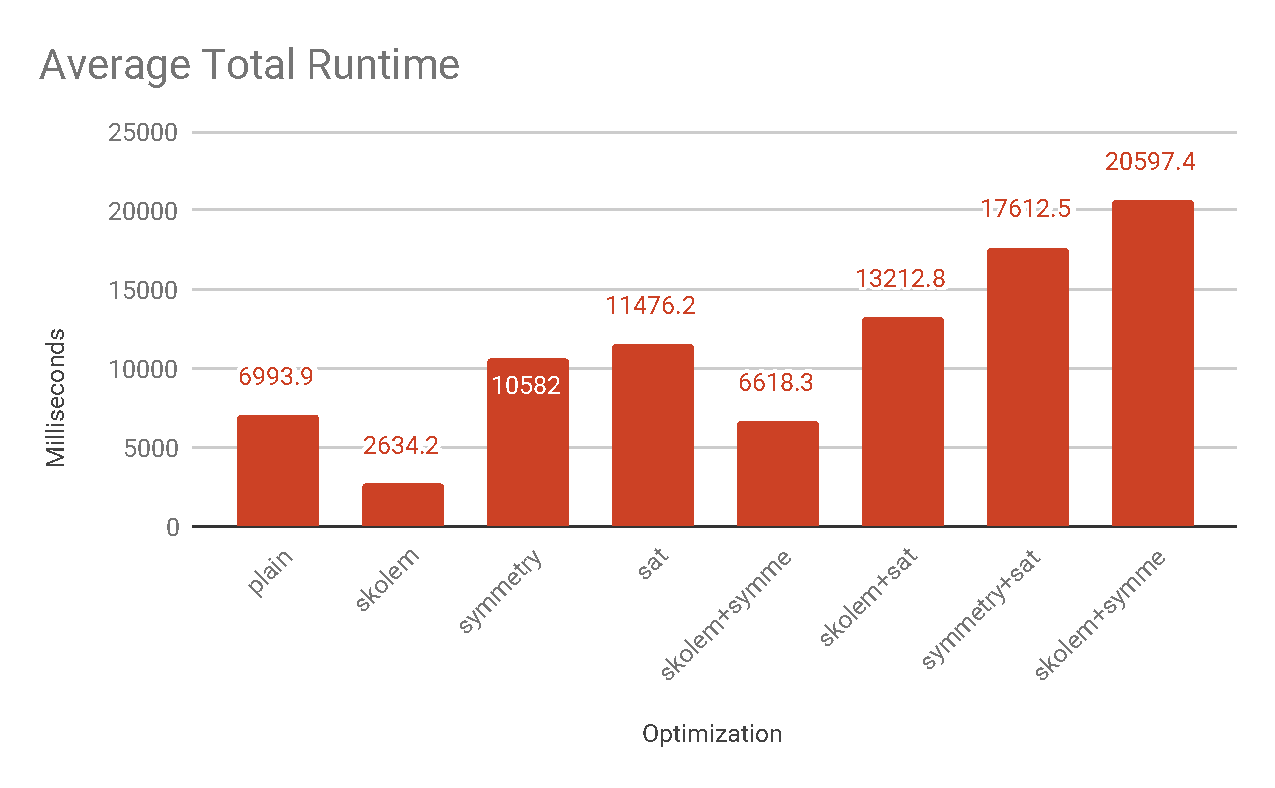
\includegraphics[width=\textwidth]{avg_total.pdf}   
      \end{minipage}\hfill
      \begin{minipage}{.5\textwidth}
        \centering
        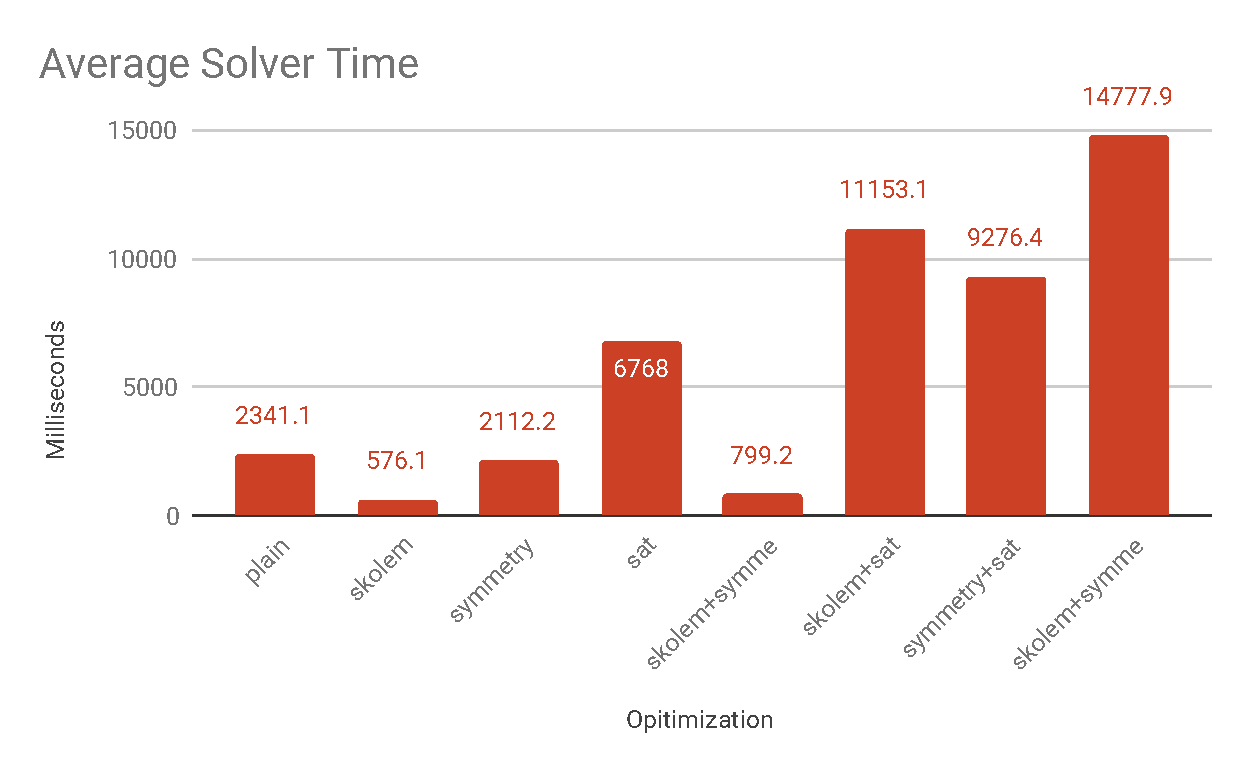
\includegraphics[width=\textwidth]{avg_solver.pdf}   
      \end{minipage}
      \caption{Averages.}
      \label{fig:averages}
    \end{figure}

    \begin{figure}[h]
      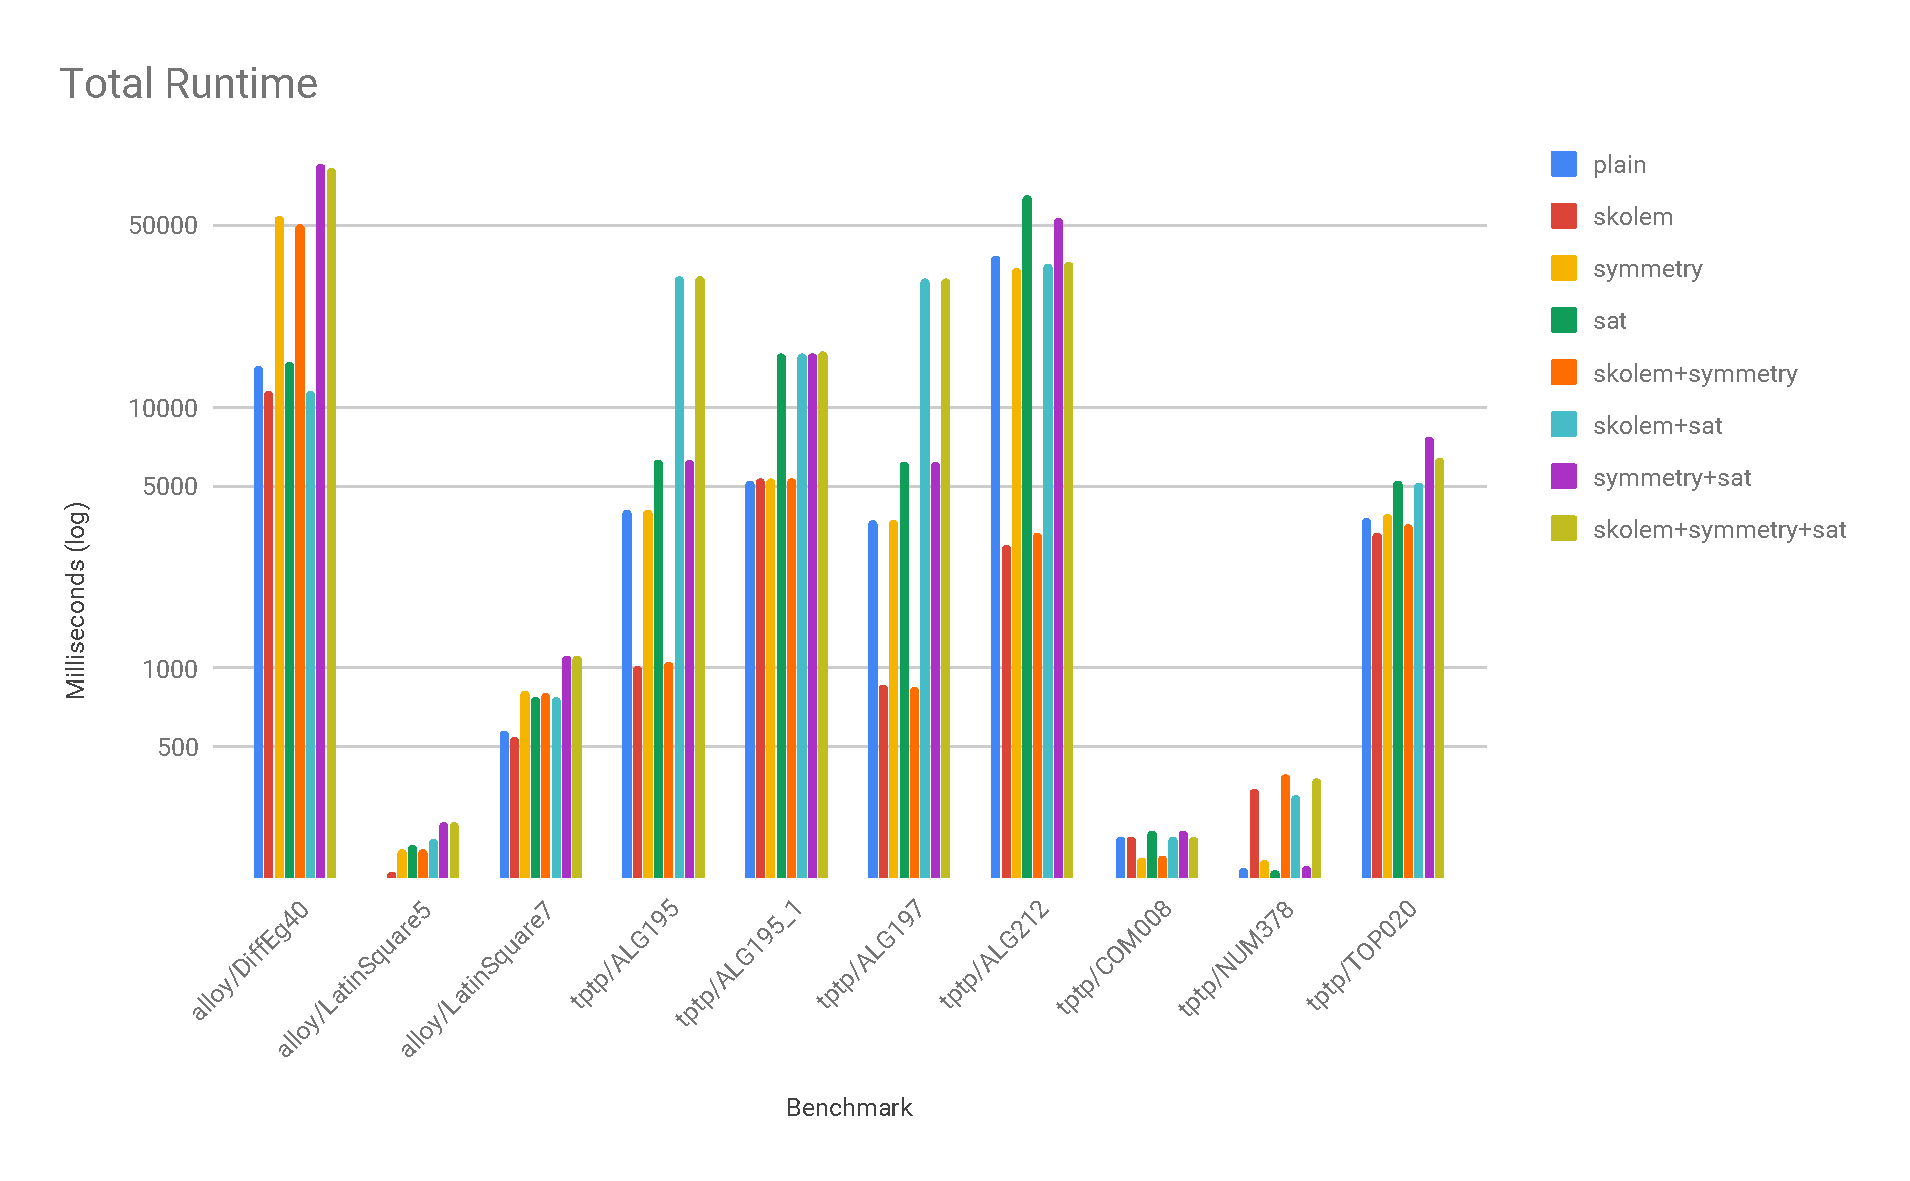
\includegraphics[width=\textwidth]{total.pdf}
      \caption{Total Times.}
      \label{fig:total}
    \end{figure}

    % \begin{figure}[h]
    %   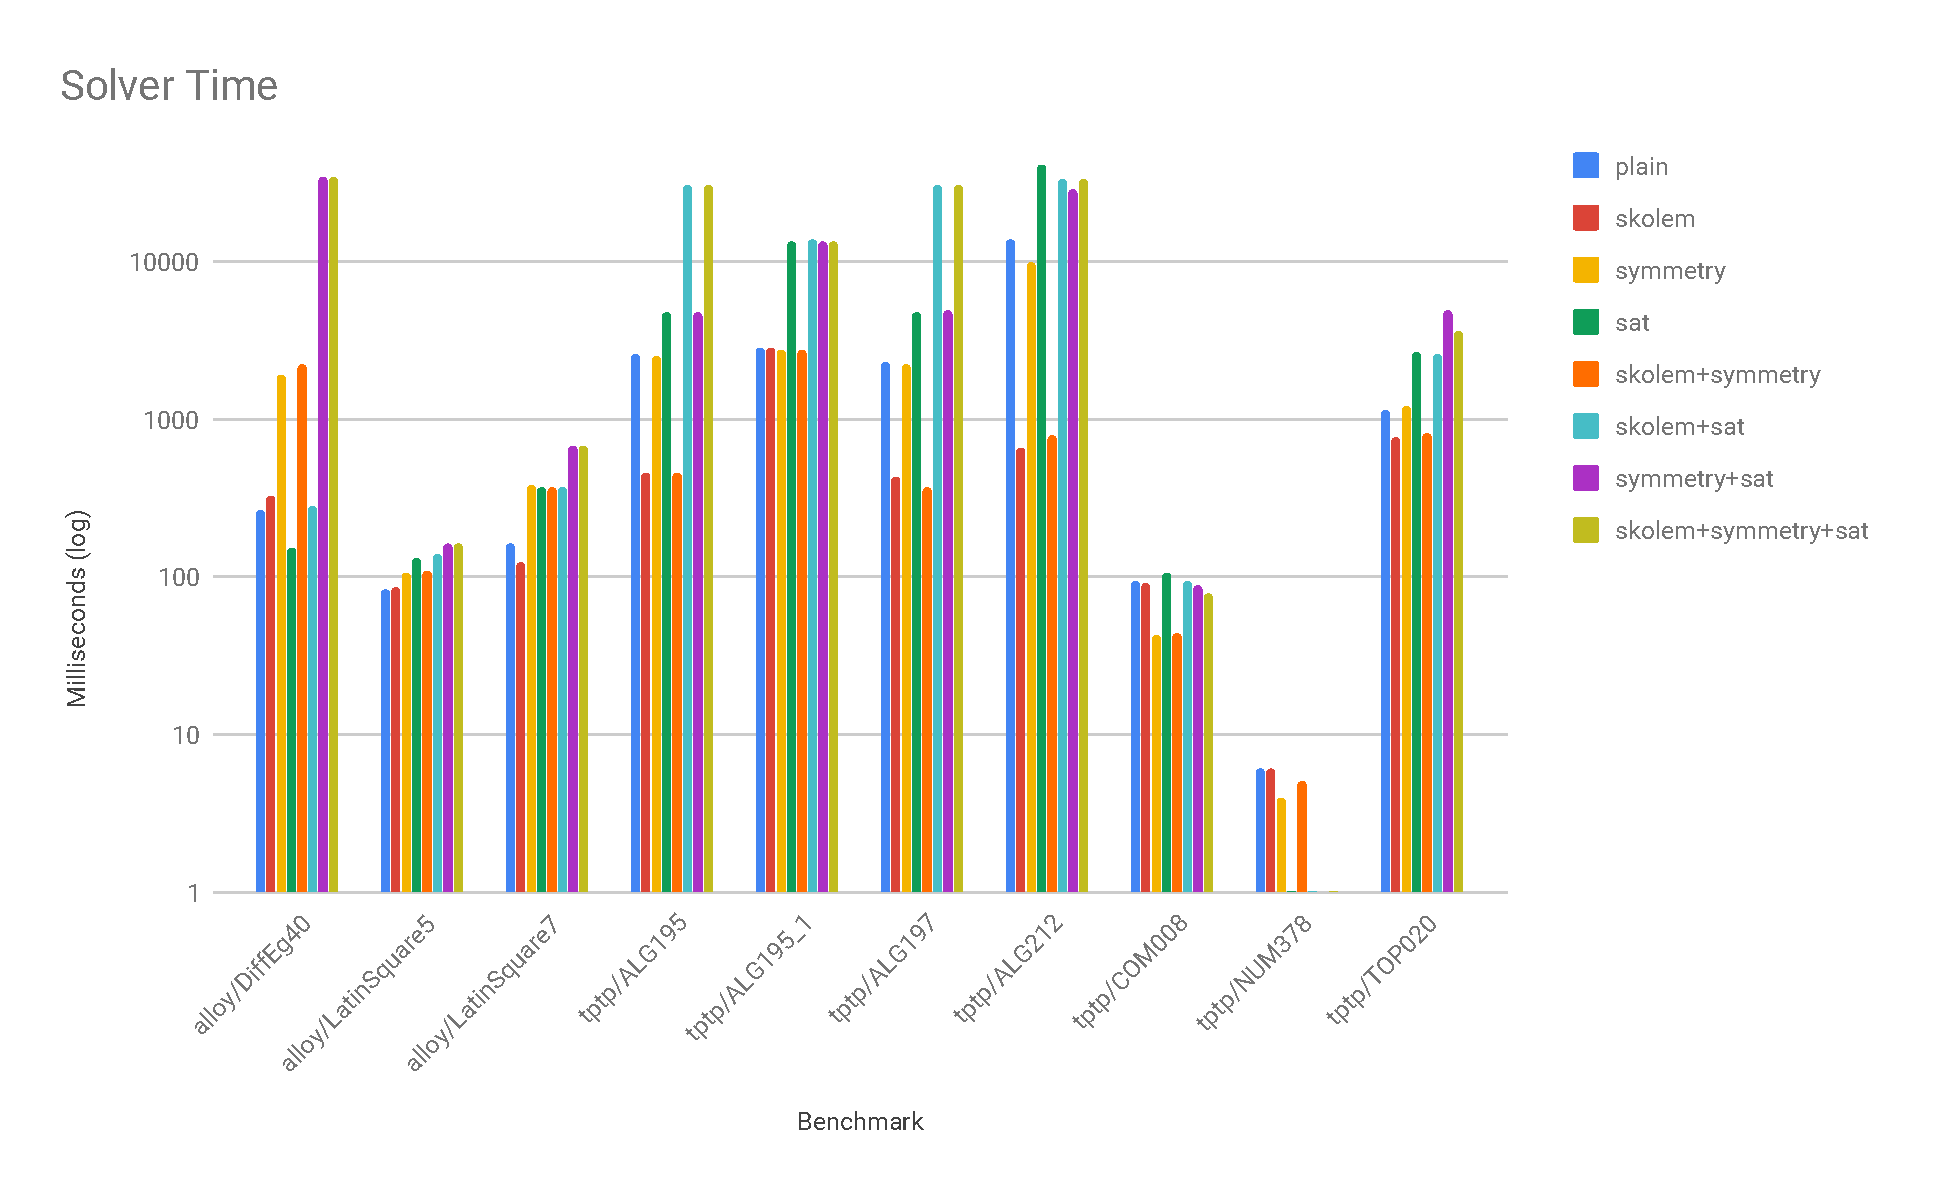
\includegraphics[width=\textwidth]{solver.pdf}
    %   \caption{Solver Times}
    %   \label{fig:solver}
    % \end{figure}

    \subsection{Project Potential}

    We see significant improvement in performance with the application of skolemization. Further investigation is required to see why symmetry breaking and translation to CNF do not improve results. In particular, we conjecture that the CNF translation works better in Kodkod due to its conjunction with circuit compaction. Answering these questions and addressing our findings would be a significant step towards a conference paper.

    We believe that if we managed to get the performance improvement we hoped for from these two optimizations, implemented a compact boolean circuit representation within Ocelot, and addressed limitations in its expressiveness, then Colocolo would become a robust and expressive tool. In particular, if we could achieve the same performance as Kodkod, Colocolo would provide a much more versatile embedding of Alloy than is possible in Java, which would open up many new possibilities for exploration and experimentation in relational logic.

  \section{Member Contributions}

  Thomas took the lead on understanding Kodkod's implementation of skolemization and translating it into an equivalent algorithm over Colocolo's AST. Altan translated Kodkod's algorithm for reducing a boolean formula to CNF and created a translator from Kodkod's AST to that of Colocolo. Both Thomas and Altan spent time testing and fixing bugs in all parts of the project as well as running benchmarks.

  \section{Course Topics}

  Colocolo touched on most of the core topics that were covered in the course (though less from the applications seen towards the second half). The most important topics we drew from were \textbf{Bounded Model Checking} and \textbf{Relational Logic} in \textbf{Alloy} and of course \textbf{Rosette}. The project itself is a \textbf{Bounded Model Finder} written on top of \textbf{Rosette}---about half the course involved gaining proficiency in Rosette and an entire lecture was spent talking about \textbf{Bounded Model Finding}. Additionally, we applied knowledge gained about \textbf{SAT Solvers} and \textbf{SMT Solvers} in our translation to CNF and comparison to \textbf{Z3}.

  The only topic we did not talk about in detail was \textbf{Skolemization}. We briefly touched on it but did not talk about any sort of implementation. Of course, our project involved a much deeper dive into the aforementioned topics than we had in class but this is to be expected. The biggest example were the details of \textbf{Alloy's Relational Logic}, which were only briefly discussed in lecture and clear, extensive documentation was difficult to find. Again, this is to be expected, the point of the course is to have a starting point to jump off from. Overall, the course provided us with the skills we needed to be able to get started and have a good idea of what direction we needed to go.

  \clearpage
  \begin{thebibliography}{999}
      \bibitem{abdulla00}
        Abdulla, P.A., Bjesse, P and Een, N.:
        \emph{Symbolic reachability analysis based on sat-solvers}
        (TACAS'00).
     \bibitem{aloul03}
        Aloul, Fadi A. and Sakallah, Karem A. and Markov, Igor L.:
        \emph{Efficient Symmetry Breaking for Boolean Satisfiability}
        Proceedings of the 18th International Joint Conference on Artificial Intelligence, (IJCAI'03).
      \bibitem{andersen97}
        Andersen, H.R. and Hulgaard, H.:
        \emph{Boolean expression diagrams}
        (LICS'97).
      \bibitem{bornholdt17}
        Bornholdt, James and Torlak, Emina:
        \emph{Synthesizing Memory Models from Framework Sketches and Litmus Tests},
        Proceedings of the 38th ACM SIGPLAN Conference on Programming Language Design and Implementation (PLDI'17).
      \bibitem{biere17}
        Biere, Armin:
        \emph{CaDiCaL, Lingeling, Plingeling, Treengeling, YalSAT Entering the SAT Competition 2017}, Proc. of SAT Competition 2017 -- Solver and Benchmark Descriptions.
      \bibitem{claessen03}
        Claessen, Koen and S{\"o}rensson:
        \emph{New Techniques that Improve {MACE}-style Model Finding}
        Proceedings of Workshop on Model Computation (MODEL'03).
      \bibitem{torlak07}
        Torlak, Emina and Jackson, Daniel:
        \emph{Kodkod: A Relational Model Finder},
        Proceedings of the 13th International Conference on Tools and Algorithms for the Construction and Analysis of Systems (TACAS'07).
    \end{thebibliography}
\end{document}
 